\documentclass[12pt, final]{extarticle}

% SECTION Paquetes
\usepackage{blindtext}
\usepackage{geometry}
\usepackage{minted}
\usepackage{lmodern}
\usepackage{caption}
\usepackage{subcaption}
\usepackage[spanish]{babel}
\usepackage[T1]{fontenc}
\usepackage{csquotes}
\usepackage{amsmath}
\usepackage{gensymb}
\usepackage[dvipsnames]{xcolor}
\usepackage{graphicx}
\usepackage[hidelinks]{hyperref}

% SECTION Configuraciones y macros
\geometry{top=3cm, bottom=2.8cm, left=2.6cm, right=2.6cm}

\graphicspath{{Media}}

\definecolor{bg}{gray}{0.97}
\usemintedstyle{manni}
\setminted{linenos, frame=lines, bgcolor=bg}

\renewcommand{\abstractname}{Resumen}

% SECTION Datos del título
\title{ADA 5\\
\textsc{Animación y Simulación del Mecanismo 4R-3E}}
\author{J. Ayil, C. Canul, E. Chablé, F. Sánchez, S. Tuyú\\
{Facultad de Ingeniería, Universidad Autónoma de Yucatán}}
\date{}

% SECTION Comenzar documento
\begin{document}
\maketitle

\begin{abstract}
    \blindtext
\end{abstract}

\section{Análisis cinemático}
\subsection{Método trigonométrico}
Felipe pipe lo está escribiendo.

\begin{figure}[ht]
    \centering
    \begin{subfigure}[b]{0.45\textwidth}
        \centering
        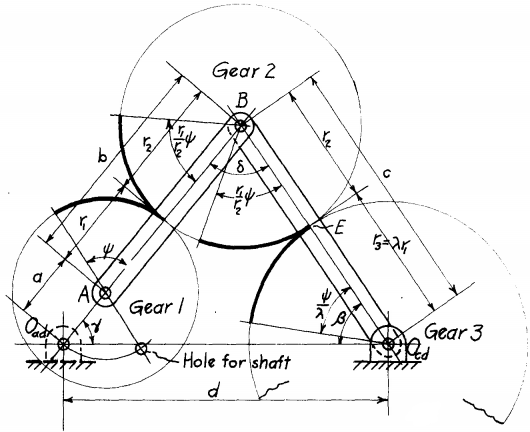
\includegraphics[width=\textwidth]{MT_1a}
        \caption{}
        \label{Fig: Los tres engranajes de transmision a}
    \end{subfigure}
    \hfill
    \begin{subfigure}[b]{0.45\textwidth}
        \centering
        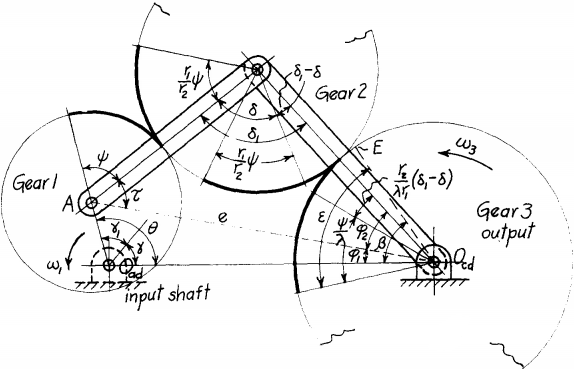
\includegraphics[width=\textwidth]{MT_2a}
        \caption{}
        \label{Fig: Los tres engranajes de transmision b}
    \end{subfigure}
    \caption{Los tres engranajes de transmisión.}
    \label{Fig: Los tres engranajes de transmision}
\end{figure}

Cuando las barras $a$ y $b$ están en una línea recta como se muestra en la
figura \ref{Fig: Los tres engranajes de transmision a}, los ángulos del
triángulo resultante son $\beta$, $\gamma$ y $\delta$. Deje
\begin{equation}
    s = \frac{1}{2}(a + b + c + d)
\end{equation}
Por trigonometría
\begin{align}
    \cos^2 \frac{\delta}{2} &= \frac{s(s - d)}{(a + b)c} \\
    \cos \delta &= 2\cos^2 \frac{\delta}{2} - 1 = \frac{2s(s - d)}{(a + b)c} - 1
\end{align}
Por teorema de senos
\begin{align}
    \sin \gamma &= \frac{c}{d}\sin\gamma \\
    \beta &= 180\degree - (\gamma + \delta)
\end{align}

Con las uniones en las posiciones de la figura
\ref{Fig: Los tres engranajes de transmision a}, deje que el eje de
transmisión en $O_{ad}$ sea removido, y deje al engrane 1 ser rotado a través
del ángulo $\psi$. Esto produce rotaciones en los engranes 2 y 3 como se indica
por los arcos gruesos y los ángulos designados.

Deje que los engranes 1 y 2 sean unidos al miembro $ab$, y deje que el mecanismo
sea movido de tal manera que el eje de transmisión pueda ser reconstruido en
$O_{ad}$. Las partes ahora están en los lugares mostrados en la figura
\ref{Fig: Los tres engranajes de transmision b} con el eje de transmisión
girado a través del ángulo $\gamma_{1}$. El ángulo $\delta$ es aumentado hasta
$\delta_{1}$, y la inclinación de la unión $BO_{cd}$ es cambiada por el valor
$\beta - (\phi_{1} + \phi_{2})$. Los engranes 2 y 3 sufrieron una rotación
adicional.

La ecuación para la rotación $\epsilon$ del engrane 3 es el que se presenta a
continuación.
\begin{equation}
    \theta = \gamma + \gamma_{1}
\end{equation}
Por el teorema de cosenos
\begin{equation}
    e^2 = a^2 + d^2 - 2ad\cos\theta = b^2 + c^2 - 2bc\cos\delta_{1}
\end{equation}
o
\begin{equation}
    \cos\delta_{1} = \frac{b^2 + c^2 - a^2 - d^2}{2bc} + \frac{ad}{bc}\cos\theta
    = K_{1} + K_{2}\cos\theta
    \label{Eq: cos delta1}
\end{equation}
donde
\begin{align}
    K_{1} &= \frac{b^2 + c^2 - a^2 - d^2}{2bc} \\
    K_{2} &= \frac{ad}{bc} \\
    \sin\tau &= \frac{c}{e}\sin\delta_{1} \\
    \phi_{2} &= 180 - (\delta_{1} + \tau) \\
    \sin\phi_{1} &= \frac{a}{e}\sin\theta \\
    \psi &= \theta + \phi_{1} - \tau_{1}
\end{align}
Entonces
\begin{equation}
    \epsilon = \beta - (\phi_{1} + \phi_{2})
    + \frac{r_{2}}{\lambda r_{1}}(\delta_{1} - \delta) + \frac{\psi}{\lambda}
\end{equation}

Para el caso en el que los engranes 1 y 3 tienen el mismo tamaño, $\lambda=1$,
la ecuación para $\epsilon$ se convierte
\begin{equation}
    \epsilon = \theta - \gamma - C\delta + C\delta_{1}
    \label{Eq: epsilon theta menos gamma}
\end{equation}
donde
\begin{equation}
    C = 1 + \frac{r_{2}}{r_{1}}
\end{equation}

Valores de $\epsilon$ pueden ser computador y graficados con estas ecuaciones.

\eqref{Eq: epsilon theta menos gamma} puede ser diferenciada para encontrar la
velocidad $\omega_{3}$ del eje de salida
\begin{equation*}
    \frac{d\epsilon}{dt} = \frac{d\theta}{dt} + C\frac{d\delta_{1}}{dt}
\end{equation*}
El coeficiente diferencial $\frac{d\theta}{dt}$ es igual a $\omega_{1}$, y el
coeficiente diferencial $\frac{d\delta_{1}}{dt}$ puede ser obtenido de
\eqref{Eq: cos delta1}. Entonces
\begin{equation}
    \omega_{3} = \omega_{1} \left[
        1 + \frac{K_{2}C\sin\theta}{\sin\delta_{1}}
    \right]
    \label{Eq: omega3 antes de sustituir}
\end{equation}
y la sustitución de \eqref{Eq: cos delta1} da
\begin{equation}
    \omega_{3} = \omega_{1} \left[
        1 + \frac{K_{2}C\sqrt{1-\cos^2\theta}}{1-(K_{1} + K_{2}\cos\theta)^2}
    \right]
    \label{Eq: omega3 despues de sustituir}
\end{equation}

\eqref{Eq: omega3 antes de sustituir} y \eqref{Eq: omega3 despues de sustituir}
son válidas para el caso en el que $r_{1} = r_{3}$. Diferenciarlas nuevamente
para obtener la aceleración genera una expresión demasiado inmanejable para
aplicaciones prácticas.

La velocidad angular $\omega_{3}$ del eje de salida puede, de igual manera, ser
encontrada por medio de la obtención de la pendiente de los diferentes puntos a
lo largo de la $\epsilon$-curva. Puede ser demostrado\cite{Milne1949} que
cuando las ordenadas $y_{0}$, $y_{1}$, $y_{2}$, $y_{3}$ y $y_{4}$ estén en cinco
equitativamente separados y conocidos puntos, la pendiente $y_{2}$ de la curva
en la ordenada de en medio está dada por la siguiente ecuación.
\begin{equation}
    {y_{2}}' = \frac{1}{12h}(y_{0} - 8y_{1} + 8y_{3} - y_{4})
\end{equation}
donde $h$ es el espaciado a lo largo de la abscisa. El proceso puede ser
repetido en la curva de velocidad para obtener la aceleración angular del eje de
salida.

\newpage
\subsection{Método vectorial}

\newpage
\section{Simulación}
\subsection{Método trigonométrico}

\subsection{Método vectorial}


\newpage
\section{Animación}
\subsection{Método trigonométrico}

\subsection{Método vectorial}


\nocite{*}
\vfill
\bibliographystyle{IEEEtran}
\bibliography{Referencias}

\end{document}